\chapter{Um assunto legal}\label{cap2}

\section{Introdução}\label{cap2:intro}

O modelo novo sugere que cada capítulo tenha um resumo, introdução, materiais e métodos, resultados, discussão e conclusões, mas optei por deixar o resumo de fora.

\section{Materiais e Métodos}\label{cap2:mem}

\subsection{Coleta dos organismos}\label{cap2:mem:coleta}

Você pode dividir cada seção em subseções para organizar melhor o conteúdo.

\subsection{Cultivo dos seres vivos}\label{cap2:mem:gametas}

\subsubsection{Embriões e Larvas}

Você também pode criar subsubseções caso necessário.
% Para inserir fórmulas matemáticas bonitinhas coloque $entre$.
% Note como formatar a unidade de temperatura e como utilizar o comando \nicefrac para frações.
A cultura foi mantida num ciclo de $12:12$ horas e temperatura constante de \unit[24]{°C}; a concentração final foi de $8\times10^5$ e $1\times10^6$ \nicefrac{células}{mL}.

\subsubsection{Metamorfose}

% Como o % representa um comentário e não é compilado, para fazê-lo aparecer no texto você precisa colocar uma "\" antes, como abaixo.
Apenas \unit[4]{\%} do texto está contido em subsubseções.

\subsection{Microscopia de luz}\label{cap2:mem:micro}

Subseção após a subseção com subsubseções via porta \emph{Firewire}.

\section{Resultados}\label{cap2:res}

\subsection{Primeiras figuras}\label{cap2:res:figs}

Subseções de novo, mas coloco algumas figuras para mostrar resultados (Figura~\ref{fig:last}). Outro jeito (Figura~\ref{fig:last2}).

% Veja a documentação para mais detalhes de como inserir figuras
% O texto entre [] na legenda será utilizado na lista de figuras (no preâmbulo), sendo ideal para substituir legendas maiores
\begin{figure}[htbp]
  \centering
  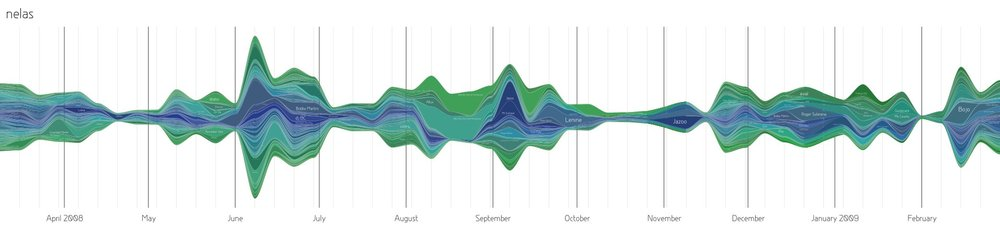
\includegraphics[width=\textwidth]{lastgraph}
  \caption[Figura simples]{Figura abstrata simples com largura igual à largura do texto.}
  \label{fig:last}
\end{figure}

\begin{figure}[htbp]
  \centering
  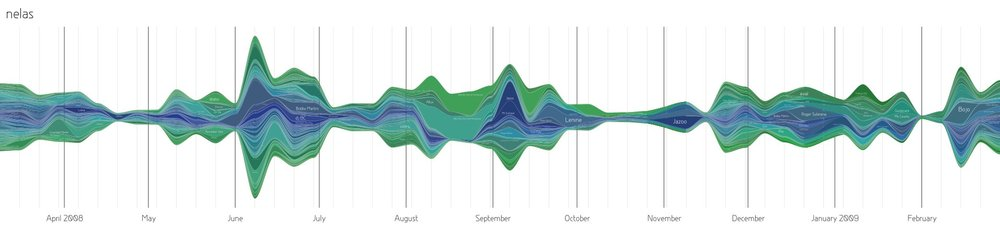
\includegraphics[width=0.5\textwidth]{lastgraph}
  \caption[Outra figura simples]{Figura abstrata simples com largura igual à metade da largura do texto.}
  \label{fig:last2}
\end{figure}

Você também pode inserir múltiplas figuras em uma só, permitindo alinhá-las de forma flexível e consistente (ver Figura~\ref{fig:fsm}).

% Note como incluir as sublegendas para cada subfigura (subfloat) e como citá-las na legenda usando o comando subref.
% Note também como incluir as referências às abreviações (nomenclature) utilizadas para que sejam listadas no preâmbulo.
\begin{figure}[htbp]
  \centering
  \subfloat[Subfigura1]{\label{fig:t1}
\includegraphics[width=200pt]{fsm}}\vspace{11pt}
  \subfloat[Subfigura2]{\label{fig:t2}
\includegraphics[width=200pt]{fsm}}\\
  \vspace{-18pt}
  \subfloat[Subfigura3]{\label{fig:t3}
\includegraphics[width=200pt]{fsm}}\vspace{11pt}
  \subfloat[Subfigura4]{\label{fig:t4}
\includegraphics[width=200pt]{fsm}}%
  \caption[Figura com subfiguras]{Exemplo de figura com subfiguras. \subref{fig:t1}~Subfigura1 (\textbf{og}) na lâmina. \subref{fig:t2}~Subfigura2 (\textbf{oppv}). \subref{fig:t3}~Subfigura3 aderida (\textbf{opv}). \subref{fig:t4}~Subfigura4. \textbf{sg}, seio genital; \textbf{ln}, lúmen.}%
  \nomenclature{og}{oogônia}%
  \nomenclature{oppv}{oócitos primários pré-vitelogênicos}%
  \nomenclature{opv}{oócitos primários vitelogênicos}%
  \nomenclature{sg}{seio genital}%
  \nomenclature{ln}{lúmen}
  \label{fig:fsm}
\end{figure}

\subsection{Tabelas}\label{cap2:res:tabs}

Utilize tabelas como a Tabela~\ref{tab:exemplo}.

% Para criar tabelas
\begin{table}[htbp]
  \caption[Tabela com \texttt{booktabs}]{Exemplo de legenda de tabela criada com o pacote \texttt{booktabs}.}
  \label{tab:exemplo}
  \vspace{1em}
  \centering
  \begin{tabular}{l r@{\,} l}
    \toprule
    Eventos     &   \multicolumn{2}{c}{Tempo}\\
    \midrule
    Entrada     &   0   &       \\
    Elevação    &   40  &   s   \\
    Corrida     &   6   &   min \\
    Saída	&   15  &   min \\
    \bottomrule
  \end{tabular}
\end{table}

% Usando o pacote units
Ocorrem no eixo \nicefrac{animal}{vegetal} (\nicefrac{A}{V}) e dividem à \unitfrac[500]{µm}{s}.
Por volta de \unit[7,5]{h} após a elevação.
% Usando o pacote nomencl
Após \unit[10]{h}, as células mesenquimais primárias (CMP) iniciam sua ingressão.%
\nomenclature{CMP}{células mesenquimais primárias}
% Colocando aspas e exemplo do pacote natbib
Larvas apresentam comportamento de ``teste de substrato''.

\section{Discussão}\label{cap2:disc}

% Comandos como o utilizado para incluir o nome da espécie estudada (subdeshort) devem ser seguidos de uma \ para inserir um espaço antes da próxima palavra. Esta \ não precisa ser utilizada quando o comando é seguido de ponto ou vírgula.
\citet{Day2006} não usaram papilas de \subsus.
% O pacote icomma permite usar a vírgula como separador decimal, já que o comportamento padrão do LaTeX é inserir um espaço maior após uma vírgula.
A migração foi similar à \subsus\ (\unitfrac[0,082]{µm}{s}).
Outro comando útil é a criação de notas de rodapé\footnote{A temperatura não foi precisada; embriões fecundados entre 25 e \unit[28]{°C}.}.
A evolução deste caráter pode ser vista de duas formas.

% Este é um dos modos de iniciar uma lista ordenada.
% Note que é possível inserir listas dentro de listas.
\begin{enumerate}
  \item{Condição inicial $\longrightarrow$ Condição final}\label{hipo:1}
    \begin{itemize}
      \item{Primeira conseqüência}
      \item{Segunda conseqüência}
    \end{itemize}
  \item{Outra condição inicial $\longrightarrow$ Condição intermediária $\longrightarrow$ Outra condição final}\label{hipo:2}
    \begin{itemize}
      \item{Conseqüência alternativa}
    \end{itemize}
\end{enumerate}

Você pode citar ítens assinalados, como a hipótese \ref{hipo:1} e a alternativa \ref{hipo:2}.

%\clearpage{\pagestyle{empty}\cleardoublepage}
